\begin{tikzpicture}[>=stealth]
    % Stavy
    \initialstate{q0}{(0,0)}{$q_0$}{(-1.2,0)}{west}
    \acceptingstate{q1}{(2.2,0)}{$q_1$}
    \state{q2}{(4.4,0)}{$q_2$}
    \acceptingstate{q3}{(6.6,0)}{$q_3$}

    % Přechody
    \transitionarrow{q0}{above}{$0,\dots,9$}{q1}
    \transitionarrow[loop above]{q1}{above}{$0,\dots,9$}{q1}
    \transitionarrow{q1}{above}{$.$}{q2}
    \transitionarrow{q2}{above}{$0,\dots,9$}{q3}
    \transitionarrow[loop above]{q3}{above}{$0,\dots,9$}{q3}
\end{tikzpicture}